\chapter{Auswertung den Ergebnissen}
\label{ch:Auswertung den Ergebnissen}
Anhand vorgeschlagene in dem Teil \ref{ch:Änderungen durch neue Antriebe, Annahmen und Methodik} Methodik wurde den Vergleich 
zwischen Referenz-Flugzeugen und alternativen Antrieben geschaffen.
Außerdem werden aufgestellte Betriebsszenarien ausgewertet und schließlich diskutiert.

\section{Ergebnisse des Gegenüberstellens von Referenzflugzeugen und neuartigen Antriebsansätzen}
%
\textbf{Vergleich des Batterie-Antriebs und SAF mit einem konventionellen Treibstoff für eine Kurzstrecke}
%
In der Abbildung \ref{vergleichBA_Ref} sind die Ergebnisse für batteriebetriebenes ES-19 und konventionelles L410 dargestellt.
Die Werte wurden für 400 Kilometer Flug bestimmt.
Die Gesamtbetriebskosten des ES-19 sind ca. 22 \% höher des konventionellen L410. Entgelte und Gebühre bewirken den größten Teil der Betriebskosten
beider Flugzeugen. Kapitalbezogene Kosten bei BA sind 36 \% höher. Der Anteil der Treibstoff- bzw. Energiekosten ist am niedrigsten 
im Vergleich zu anderen Kosten und mit einem Trend, dass die Treibstoffkosten sind bei konventionellem Flugzeug 30 \% höher.
\begin{figure}[h]
	\centering
	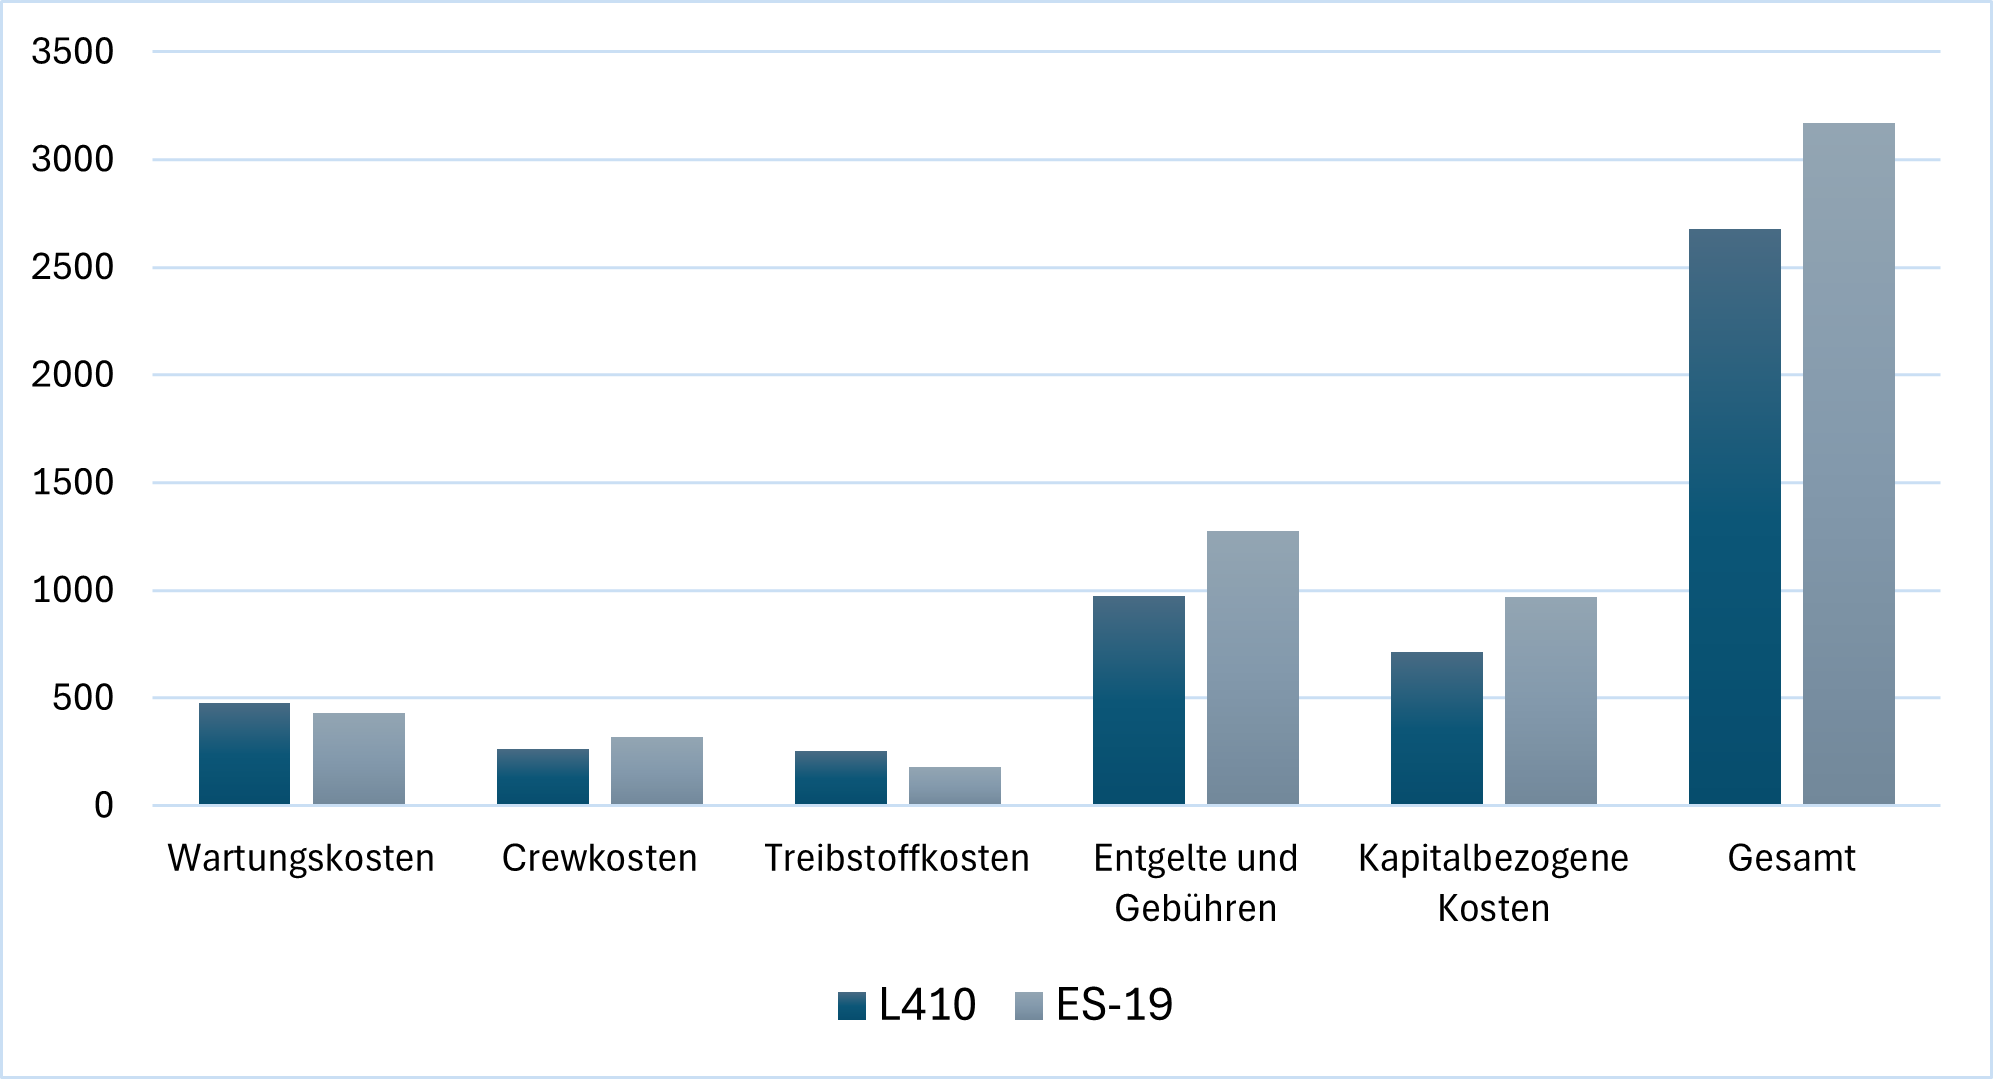
\includegraphics[width=0.9\linewidth]{Bilder/VergleichBA_Ref.png}
	\caption[Betriebskosten]{Vergleich der Referenz und Flugzeug mit der Batterie-Antrieb}
	\label{vergleichBA_Ref}
\end{figure}

\textbf{Vergleich des Wasserstoffantriebs und SAFs mit einem Referenzflugzeug für eine Mittelstrecke}
In der vorgeschlagene Vorgehensweise wurde den Vergleich zwischen den herkömmlichen Treibstoffen
und durch Wasserstoffturbine betriebenen Flugzeug, als auch mit SAF für 6000 Kilometer-Flug geschaffen. %satz übelstschlecht

